% =====================================================================
% Snippet: radar-chart.tex
% =====================================================================
% USAGE: Radar (spider) chart with 5-6 axes for multi-dimensional
% model comparison. Useful when comparing 2-3 methods on multiple
% benchmarks at once.
%
% Copy %% COPY-START / END, replace:
%   - axes: list of axis labels (5-6 recommended)
%   - data: scores 0-100 for each axis
%   - 1 or 2 polygons (compare 2 methods)
% =====================================================================

\documentclass[tikz,border=10pt]{standalone}
\usepackage{xcolor,tikz,amssymb}
\usetikzlibrary{positioning,calc}

\definecolor{acaBlueLine}{HTML}{3060A8}
\definecolor{acaBlueFill}{HTML}{6890C8}
\definecolor{acaOrangeLine}{HTML}{D06020}
\definecolor{acaOrangeFill}{HTML}{F08850}
\definecolor{acaGreyLine}{HTML}{606060}

\begin{document}
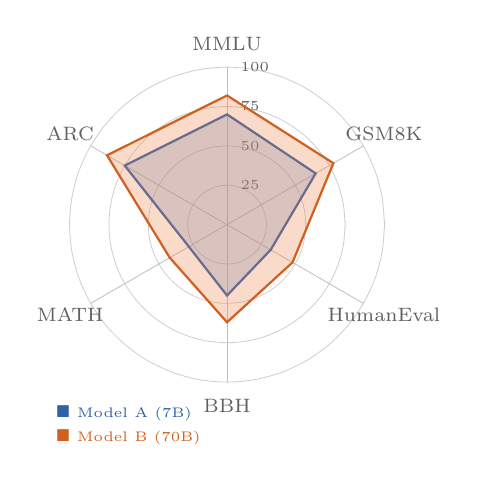
\begin{tikzpicture}

%% COPY-START =========================================================

\def\xC{0}
\def\yC{0}
\def\rad{2.0}              % max radius
\def\nAxes{6}              % number of axes

% --- AXIS LABELS (positioned at radius * 1.15) ---
\def\axisLabels{MMLU, GSM8K, HumanEval, BBH, MATH, ARC}

% --- DATA (0-100 for each axis), 2 models ---
\def\dataModelA{70, 65, 32, 45, 28, 75}    % Model A (e.g., 7B)
\def\dataModelB{82, 78, 48, 62, 42, 88}    % Model B (e.g., 70B)

% --- DRAW CONCENTRIC GRID (25/50/75/100%) ---
\foreach \r in {0.25, 0.5, 0.75, 1.0} {
  \pgfmathsetmacro\rPos{\rad * \r}
  \draw[acaGreyLine!30, line width=0.3pt]
    plot[domain=0:360, samples=37, smooth cycle]
      ({\xC + \rPos * cos(\x)}, {\yC + \rPos * sin(\x)});
}
\foreach [count=\j] \r in {25, 50, 75, 100} {
  \pgfmathsetmacro\rPos{\rad * \r / 100}
  \node[anchor=west, font=\tiny, color=acaGreyLine]
    at (\xC + 0.05, \yC + \rPos) {\r};
}

% --- DRAW AXES (radial lines + labels) ---
\foreach [count=\i] \lab in \axisLabels {
  \pgfmathsetmacro\ang{90 - 360 * (\i - 1) / \nAxes}
  \pgfmathsetmacro\ex{\xC + \rad * cos(\ang)}
  \pgfmathsetmacro\ey{\yC + \rad * sin(\ang)}
  \draw[acaGreyLine!40, line width=0.3pt] (\xC, \yC) -- (\ex, \ey);
  \pgfmathsetmacro\lx{\xC + \rad * 1.15 * cos(\ang)}
  \pgfmathsetmacro\ly{\yC + \rad * 1.15 * sin(\ang)}
  \node[font=\scriptsize, color=acaGreyLine]
    at (\lx, \ly) {\lab};
}

% --- DRAW MODEL A POLYGON (compute coords first, then chain) ---
\foreach [count=\i] \val in \dataModelA {
  \pgfmathsetmacro\ang{90 - 360 * (\i - 1) / \nAxes}
  \pgfmathsetmacro\rr{\rad * \val / 100}
  \pgfmathsetmacro\px{\xC + \rr * cos(\ang)}
  \pgfmathsetmacro\py{\yC + \rr * sin(\ang)}
  \coordinate (pa\i) at (\px, \py);
}
\draw[acaBlueLine, fill=acaBlueFill, fill opacity=0.3, line width=0.8pt]
  (pa1) -- (pa2) -- (pa3) -- (pa4) -- (pa5) -- (pa6) -- cycle;

% --- DRAW MODEL B POLYGON ---
\foreach [count=\i] \val in \dataModelB {
  \pgfmathsetmacro\ang{90 - 360 * (\i - 1) / \nAxes}
  \pgfmathsetmacro\rr{\rad * \val / 100}
  \pgfmathsetmacro\px{\xC + \rr * cos(\ang)}
  \pgfmathsetmacro\py{\yC + \rr * sin(\ang)}
  \coordinate (pb\i) at (\px, \py);
}
\draw[acaOrangeLine, fill=acaOrangeFill, fill opacity=0.3, line width=0.8pt]
  (pb1) -- (pb2) -- (pb3) -- (pb4) -- (pb5) -- (pb6) -- cycle;

% --- LEGEND ---
\node[anchor=west, font=\tiny, color=acaBlueLine]
  at (\xC - \rad - 0.3, \yC - \rad - 0.4) {$\blacksquare$ Model A (7B)};
\node[anchor=west, font=\tiny, color=acaOrangeLine]
  at (\xC - \rad - 0.3, \yC - \rad - 0.7) {$\blacksquare$ Model B (70B)};

%% COPY-END ===========================================================

\end{tikzpicture}
\end{document}
